%
% kommutator.tex -- Kommutator von T_b und D_a
%
% (c) 2019 Prof Dr Andreas Müller, Hochschule Rapperswil
%
\documentclass[tikz]{standalone}
\usepackage{amsmath}
\usepackage{times}
\usepackage{txfonts}
\usepackage{pgfplots}
\usepackage{csvsimple}
\usetikzlibrary{arrows,intersections,math}
\begin{document}
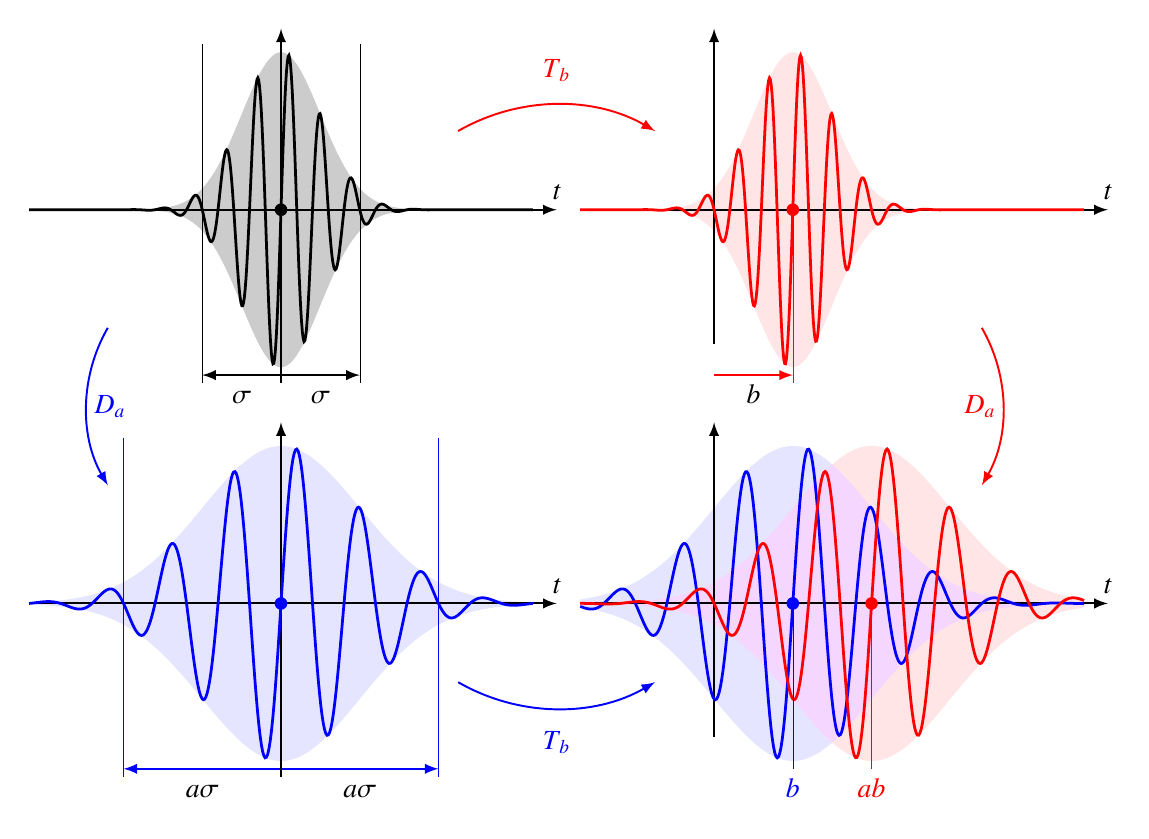
\begin{tikzpicture}[>=latex]

\def\a{2}
\def\b{1}
\def\pivalue{3.14159}
\def\frequency{5*\pivalue}

\def\steps{600}

\begin{scope}[xshift=-3.5cm,yshift=2.5cm]
\fill[color=gray!40]
	plot[domain=-3.2:3.2,samples={\steps}]
		({\x},{2*exp(-\x*\x*2))}) --
	plot[domain=3.2:-3.2,samples={\steps}]
		({\x},{-2*exp(-\x*\x*2))}) -- cycle;
\draw[line width=0.1pt] (-1,2.1)--(-1,-2.2);
\draw[line width=0.1pt] (1,2.1)--(1,-2.2);
\draw[<->,line width=0.7pt] (-1,-2.1)--(1,-2.1);
\node at (0.5,-2.1) [below] {$\sigma\mathstrut$};
\node at (-0.5,-2.1) [below] {$\sigma\mathstrut$};
\draw[->,line width=0.7pt] (-3.2,0)--(3.5,0) coordinate[label=$t$];
\draw[->,line width=0.7pt] (0,-2.2)--(0,2.3);
\draw[line width=1pt] plot[domain=-3.2:3.2,samples={\steps}]
	({\x},{2*exp(-\x*\x*2)*sin(\frequency*\x*(180/\pivalue)});
\fill (0,0) circle[radius=0.08];
\end{scope}

%
% Wirkung von T_b
%
\begin{scope}[xshift=2cm,yshift=2.5cm]
\fill[color=red!10]
	plot[domain=-1.7:4.7,samples={\steps}]
		({\x},{2*exp(-(\x-\b)*(\x-\b)*2))}) --
	plot[domain=4.7:-1.7,samples={\steps}]
		({\x},{-2*exp(-(\x-\b)*(\x-\b)*2))}) -- cycle;
\draw[->,color=red,line width=0.7pt] (0,-2.1)--({\b},-2.1);
\draw[line width=0.1pt,color=red] ({\b},0)--({\b},-2.2);
\node at ({\b/2},-2.1) [below] {$b\mathstrut$};
\draw[->,line width=0.7pt] (-1.7,0)--(5,0) coordinate[label=$t$];
\draw[->,line width=0.7pt] (0,-1.7)--(0,2.3);
\draw[line width=1pt,color=red] plot[domain=-1.7:4.7,samples={\steps}]
	({\x},{2*exp(-(\x-\b)*(\x-\b)*2)*sin(\frequency*(\x-\b)*(180/\pivalue)});
\fill[color=red] (\b,0) circle[radius=0.08];
\end{scope}

\def\steps{400}

%
% Wirkung von D_a
%
\begin{scope}[xshift=-3.5cm,yshift=-2.5cm]
\fill[color=blue!10]
	plot[domain={-3.2}:{3.2},samples={\steps}]
		({\x},{2*exp(-(\x/\a)*(\x/\a)*2)}) --
	plot[domain={3.2}:{-3.2},samples={\steps}]
		({\x},{-2*exp(-(\x/\a)*(\x/\a)*2)}) -- cycle;
\draw[color=blue,line width=0.1pt] ({-\a},2.1)--({-\a},{-2.2});
\draw[color=blue,line width=0.1pt] ({\a},2.1)--({\a},{-2.2});
\draw[<->,color=blue,line width=0.7pt] ({-\a},-2.1)--({\a},-2.1);
\draw[->,line width=0.7pt] (-3.2,0)--(3.5,0) coordinate[label=$t$];
\draw[->,line width=0.7pt] (0,-2.2)--(0,2.3);
\node at ({-0.5*\a},-2.1) [below] {$a\sigma\mathstrut$};
\node at ({0.5*\a},-2.1) [below] {$a\sigma\mathstrut$};
\draw[line width=1pt,color=blue] plot[domain={-3.2}:{3.2},samples={\steps}]
	({\x},{2*exp(-(\x/\a)*(\x/\a)*2)*sin(\frequency*(\x/\a)*(180/\pivalue)});
\fill[color=blue] (0,0) circle[radius=0.08];
\end{scope}

%
% Wirkung von D_a und T_b
%
\begin{scope}[xshift=2cm,yshift=-2.5cm]
\fill[color=blue!10]
	plot[domain={-1.7}:{4.7},samples={\steps}]
		({\x},{2*exp(-((\x-\b)/\a)*((\x-\b)/\a)*2)}) --
	plot[domain={4.7}:{-1.7},samples={\steps}]
		({\x},{-2*exp(-((\x-\b)/\a)*((\x-\b)/\a)*2)}) -- cycle;
\fill[color=red!10]
	plot[domain=-1.7:4.7,samples={\steps}]
		({\x},{2*exp(-((\x/\a)-\b)*((\x/\a)-\b)*2))}) --
	plot[domain=4.7:-1.7,samples={\steps}]
		({\x},{-2*exp(-((\x/\a)-\b)*((\x/\a)-\b)*2))}) -- cycle;

\begin{scope}
\clip
	plot[domain={-1.7}:{4.7},samples={\steps}]
		({\x},{2*exp(-((\x-\b)/\a)*((\x-\b)/\a)*2)}) --
	plot[domain={4.7}:{-1.7},samples={\steps}]
		({\x},{-2*exp(-((\x-\b)/\a)*((\x-\b)/\a)*2)}) -- cycle;
\definecolor{pink}{rgb}{0.8,0.2,1}
\fill[color=pink!20]
	plot[domain=-1.7:4.7,samples={\steps}]
		({\x},{2*exp(-((\x/\a)-\b)*((\x/\a)-\b)*2))}) --
	plot[domain=4.7:-1.7,samples={\steps}]
		({\x},{-2*exp(-((\x/\a)-\b)*((\x/\a)-\b)*2))}) -- cycle;
\end{scope}

\draw[->,line width=0.7pt] (-1.7,0)--(5,0) coordinate[label=$t$];
\draw[->,line width=0.7pt] (0,-1.7)--(0,2.3);
\draw[line width=1pt,color=blue] plot[domain={-1.7}:{4.7},samples={\steps}]
	({\x},{2*exp(-((\x-\b)/\a)*((\x-\b)/\a)*2)*sin(\frequency*((\x-\b)/\a)*(180/\pivalue)});
\draw[line width=1pt,color=red] plot[domain=-1.7:4.7,samples={\steps}]
	({\x},{2*exp(-((\x/\a)-\b)*((\x/\a)-\b)*2)*sin(\frequency*((\x/\a)-\b)*(180/\pivalue)});
\fill[color=red] ({\a*\b},0) circle[radius=0.08];
\fill[color=blue] (\b,0) circle[radius=0.08];
\draw[line width=0.1pt,color=blue] ({\b},0)--({\b},-2.1);
\node[color=blue] at ({\b},-2.1) [below] {$b$};
\draw[line width=0.1pt,color=red] ({\a*\b},0)--({\a*\b},-2.1);
\node[color=red] at ({\a*\b},-2.1) [below] {$ab$};
\end{scope}

%
% Abbildungspfeile
%
\def\r{2.5}

\draw[<-,line width=0.7pt,color=red] ({\r/2},3.5) arc (60:120:\r);
\node[color=red] at (0,4) [above] {$T_b$};

\draw[<-,line width=0.7pt,color=blue] ({\r/2},-3.5) arc (-60:-120:\r);
\node[color=blue] at (0,-4) [below] {$T_b$};

\def\r{2}

\draw[->,line width=0.7pt,color=blue] (-5.7,{\r/2}) arc (150:210:\r);
\node[color=blue] at (-6,0) [right] {$D_a$};

\draw[<-,line width=0.7pt,color=red] (5.4,{-\r/2}) arc (-30:30:\r);
\node[color=red] at (5.7,0) [left] {$D_a$};

\end{tikzpicture}
\end{document}

